\subsection{Selective edge pruning} \label{s:sel_pruning}

Through the experiments performed in thisw project and the analysis in the PGCNA paper \cite{Care2019-ij} it was noticed that if a node has too many edges, the network becomes messy and more complicated to analyse. Conversely, if a node has a few edges (<3), then the community detection (Leiden \citet{Traag2019-ne}) finds disconnected community. \cite{Care2019-ij} (empirically) found that the appropriate number of edges for a node is 3, and it is the value used throughout the project for the non-transcription factor gene (or 'standard'). 

The project aims to prioritise the transcription factor (TF) over the standard genes as these genes up-regulated the expression of the other genes, thus having a higher biological importance. By allowing more connections for the TF, the minimum degree of the node increases as well as their role in the network, similar to the biology. The experiments, on selective edge pruning, aim to explore and find the appropriate minimum degree for TF genes and how varying it affects the network. The work in this section was presented as a poster at the \textit{\href{https://2023.complexnetworks.org/}{Complex Network Conference in 2023}}.

A second aim of this section is to compare the Leiden \citet{Traag2019-ne} community detection used in PGCNA with the degree corrected Stochastic Block Model (DC-SBM) from \cite{Karrer2011-si, Peixoto2017-gc}. As it was covered in \cref{s:lit:comm_detect} from Introduction, Leiden is faster and more popular, but it is prone to find patterns in noise, whereas the DC-SBM is slower but it is more error prone in find non-existent communities. The reason for comparing the two is that to decide on the next improvements to the network pipeline. Throughout the project DC-SBM was preferred over the simple SBM \cite{Holland1983-eu} as it accounts for node's degree when it finds the communities, which is crucial for selective edge pruning; for convinience DC-SBM and SBM are used interchangeably.

\subsubsection{Experiments setup}


The experiments performed in this section are using the RNAseq gene expression from TCGA's MIBC cohort from TCGA and the transcription factor list was taken from \citet{Lambert2018-el}. As before, the Kallisto method was used to align the RNA-seq reads using genome version GRCh38 with Gencode annotation version 42. The gene selection strategy for the network is followed as in \ref{} (v3- method), using 5000 most varied genes from which 325 are Transcription Factors.


%Leiden and SBM configuration
The same network pipeline as described in \cref{fig:N_I:network_pipeline} was applied. Both Leiden and DC-SBM are applied and compared in the following sections. Leiden was run using Modularity Maximisation cost function and iterate over 10 times at each run. The degree-corrected Stochastic Block Model was used, with 700 iterations ($n\_iter=700$), the entire graph was swept up to 10 times ($mc\_iter = 10 sweeps$) and the distribution of the data was set to real exponential\footnote{As in the \href{https://graph-tool.skewed.de/static/doc/demos/inference/inference.html}{Graph-tool documentation} the distribution of the edge covariance can be specified given the bounds of the data, as seen in the referenced guide.} ($distribution = real\_exponential$). The number of iterations and swept insured that a detailed search for the communities is performed while keeping the computational times low. The 'real-exponential' parameter it is used for edge weights that range from $[0, \infty]$.

% Metrics
The performance of the Leiden algorithm is measured by the Modularity Maximisation (described in \cref{s:lit:mod_max}) which measure the separation between the communities; higher values the better. In contrast, SBM performance is measured by the Minimum Description Length (MDL) which measures the minimum information needed to describe the data; i.e. lower values the better. The number of communities found by the two community detection algorithm was also used a heurestic to assess the performance; it is generally thought that more communities the better \citet{Care2019-ij}. Unfortunately, at the moment of running this experiment there was no common metric used to compare the performance of the two methods, however at the end of summer 2023 \citet{Peixoto2023-mw}, Tiago Peixto published research that adapted MDL to Modularity models (like Leiden).

%Choosing the Control TF
To account for the random effects of the TFs in the network, there are 10 control experiments with 325 non-TF randomly selected and allowed a minimum degree from 3-15. The lower bound is given by the value used by the standard genes while the higher limit was decided empirically as all the prioritised subset are used for stratification (see \cref{fig:N_I:sel_tfs}; i.e. selected as important genes and used for stratification.



\subsubsection{Community detection comparison}

\begin{figure}[!htb]   
\centering
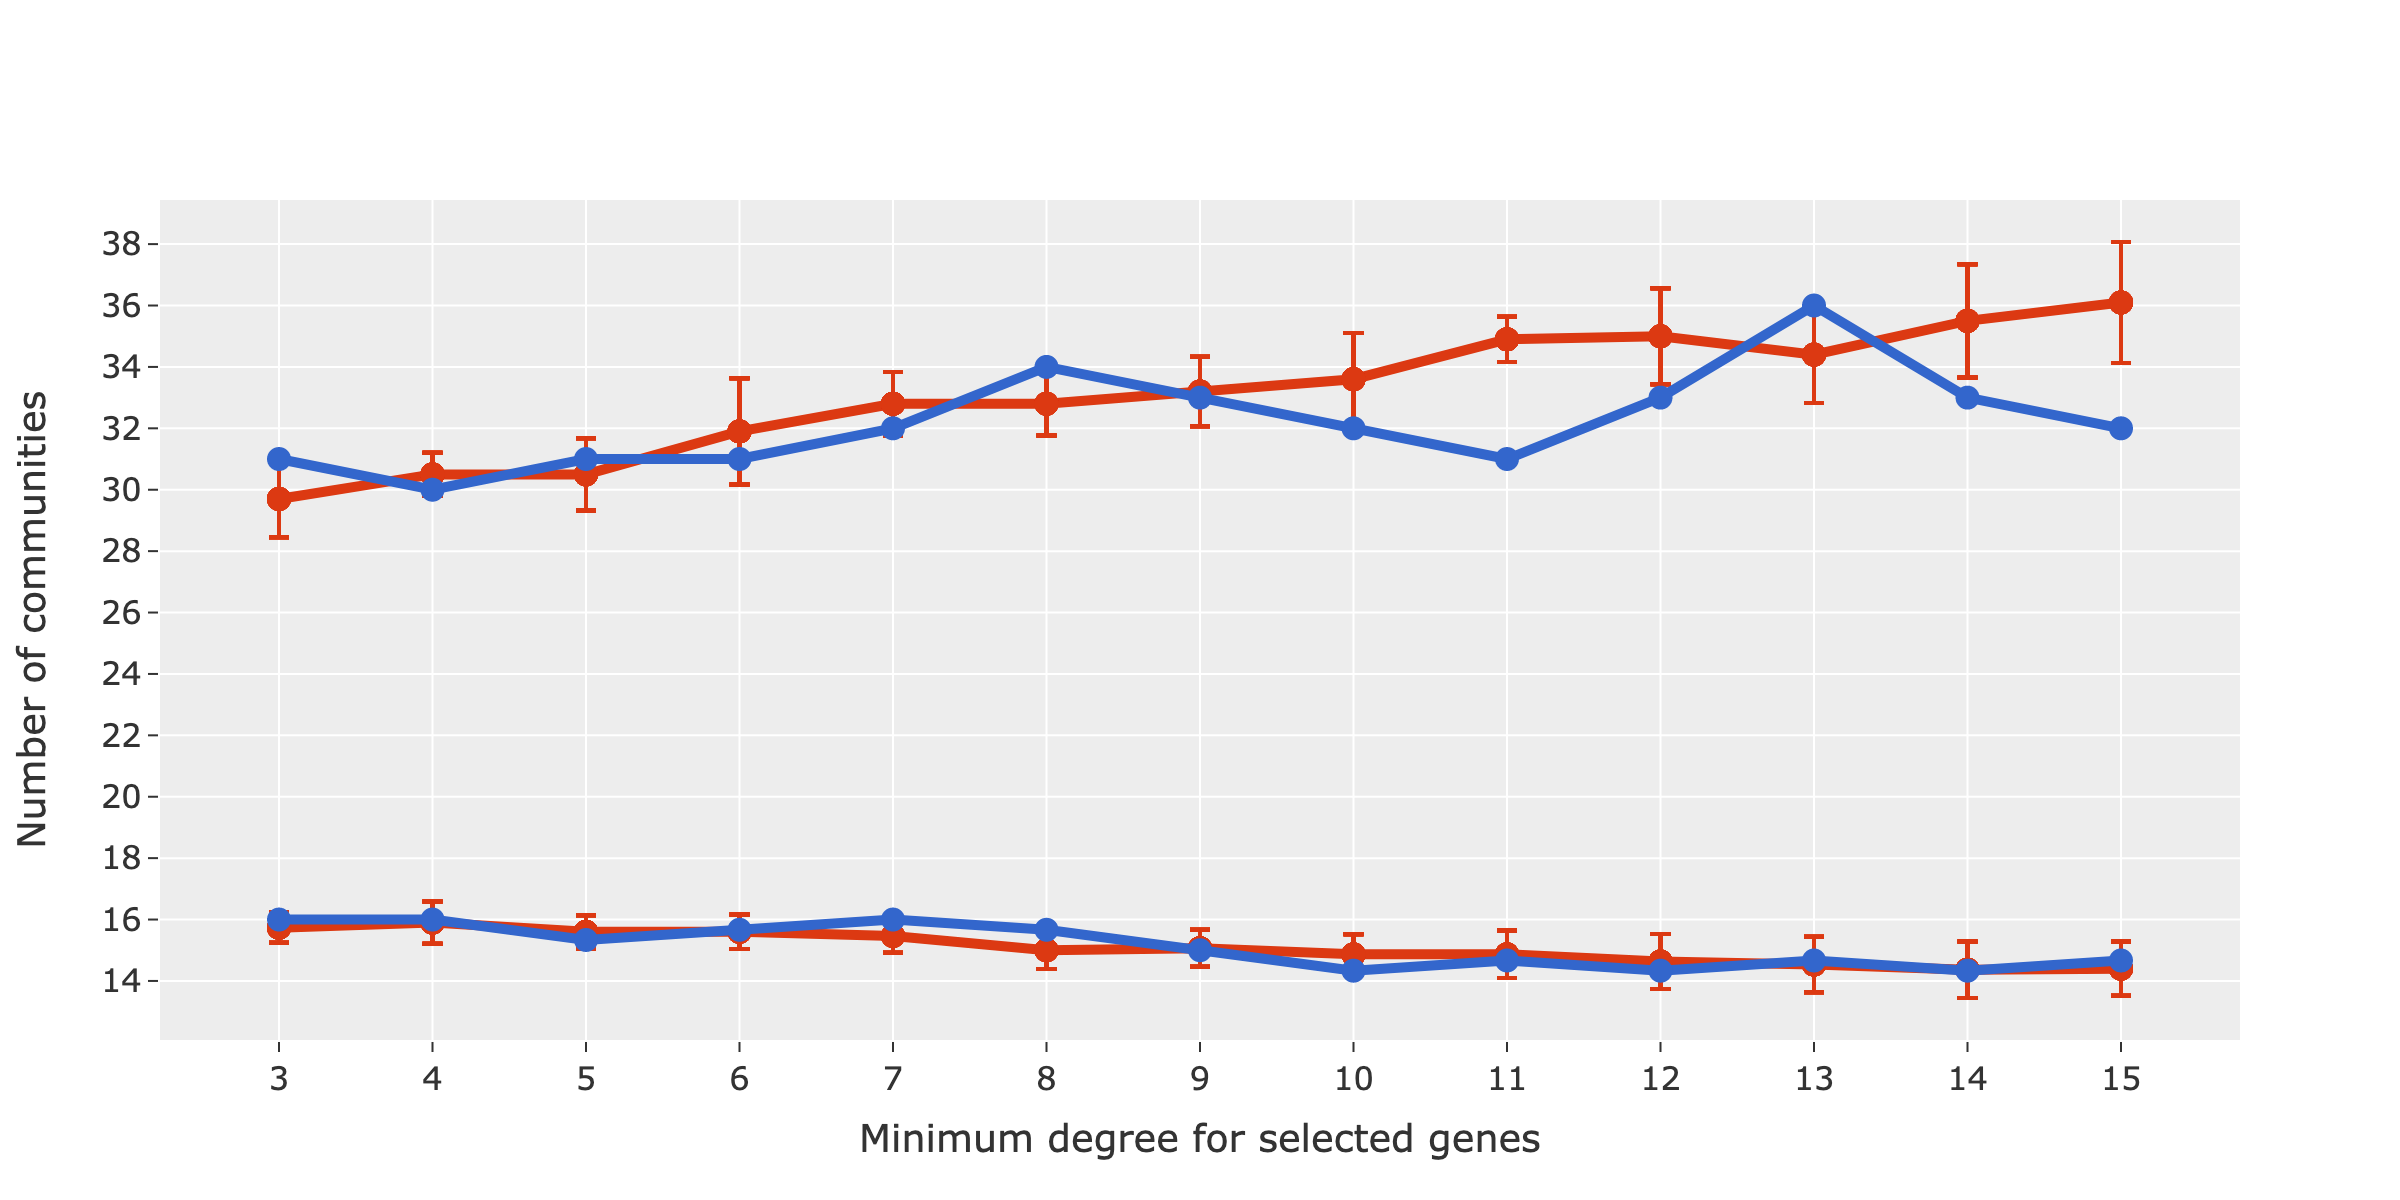
\includegraphics[width=1.0\textwidth,height=1.0\textheight,keepaspectratio]{Sections/Network_I/Resources/selective_pruning/sbm_Leiden_combNum.png}
  \caption{Community size for Leiden and Stochastic Block Model}
\label{fig:N_I:leid_mod_sel}
\end{figure}


\begin{figure}[!htb]
    \captionsetup[subfigure]{justification=Centering}
    \begin{subfigure}[!t]{1.0\textwidth}
        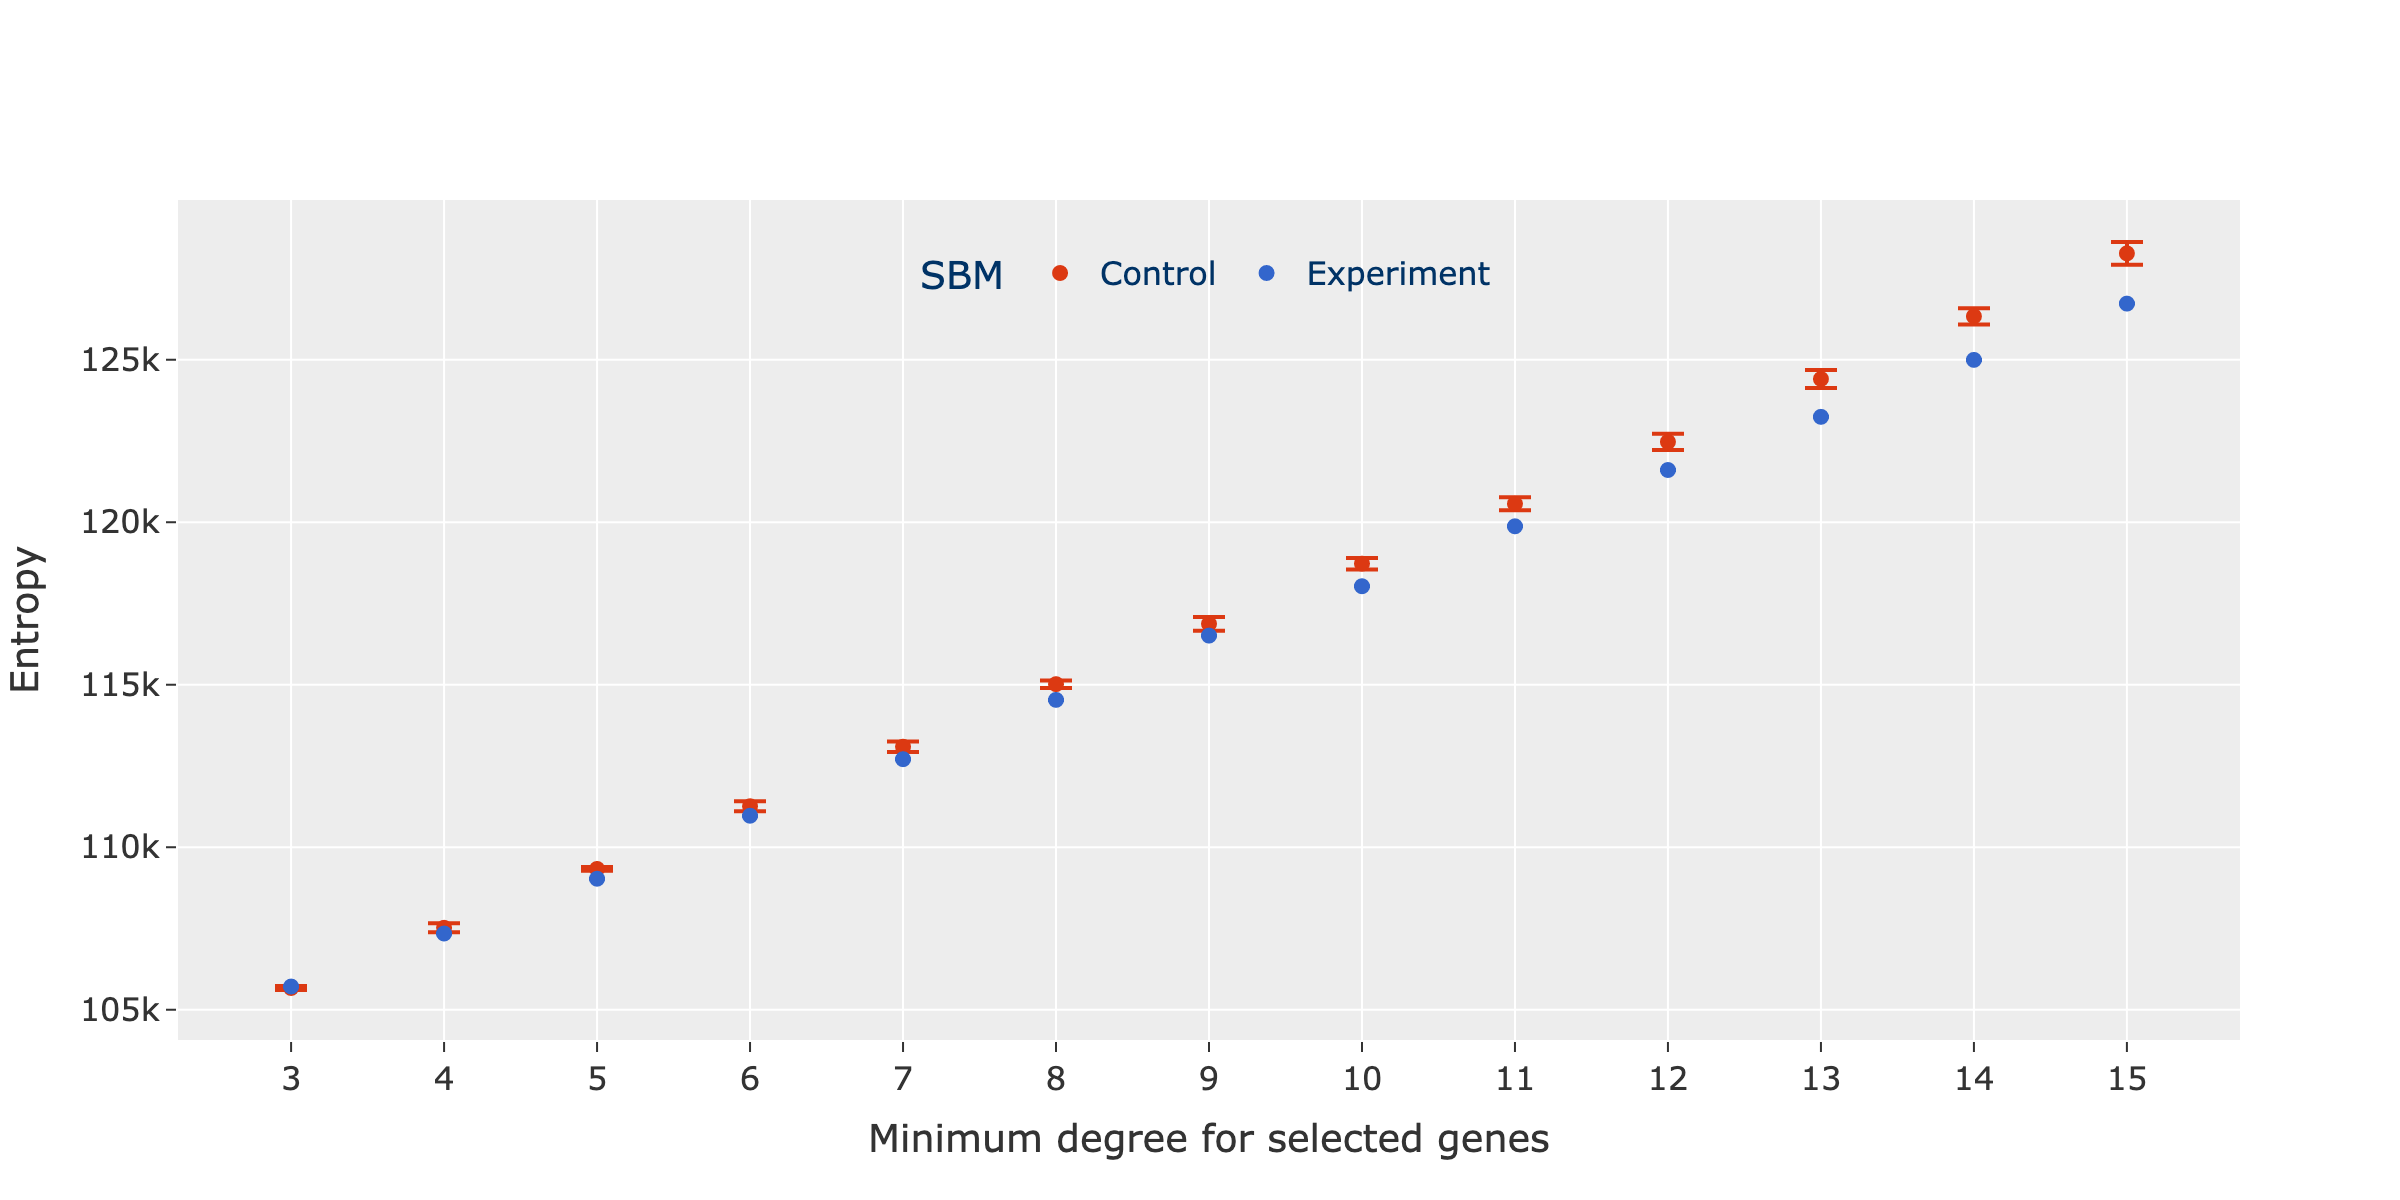
\includegraphics[width=\textwidth]{Sections/Network_I/Resources/selective_pruning/sbm_ent_sel_prun.png}
        \caption{SBM entropy}
    \end{subfigure}\hspace{\fill} % maximize horizontal separation

    \bigskip % more vertical separation
    \begin{subfigure}[!t]{1.0\textwidth}
        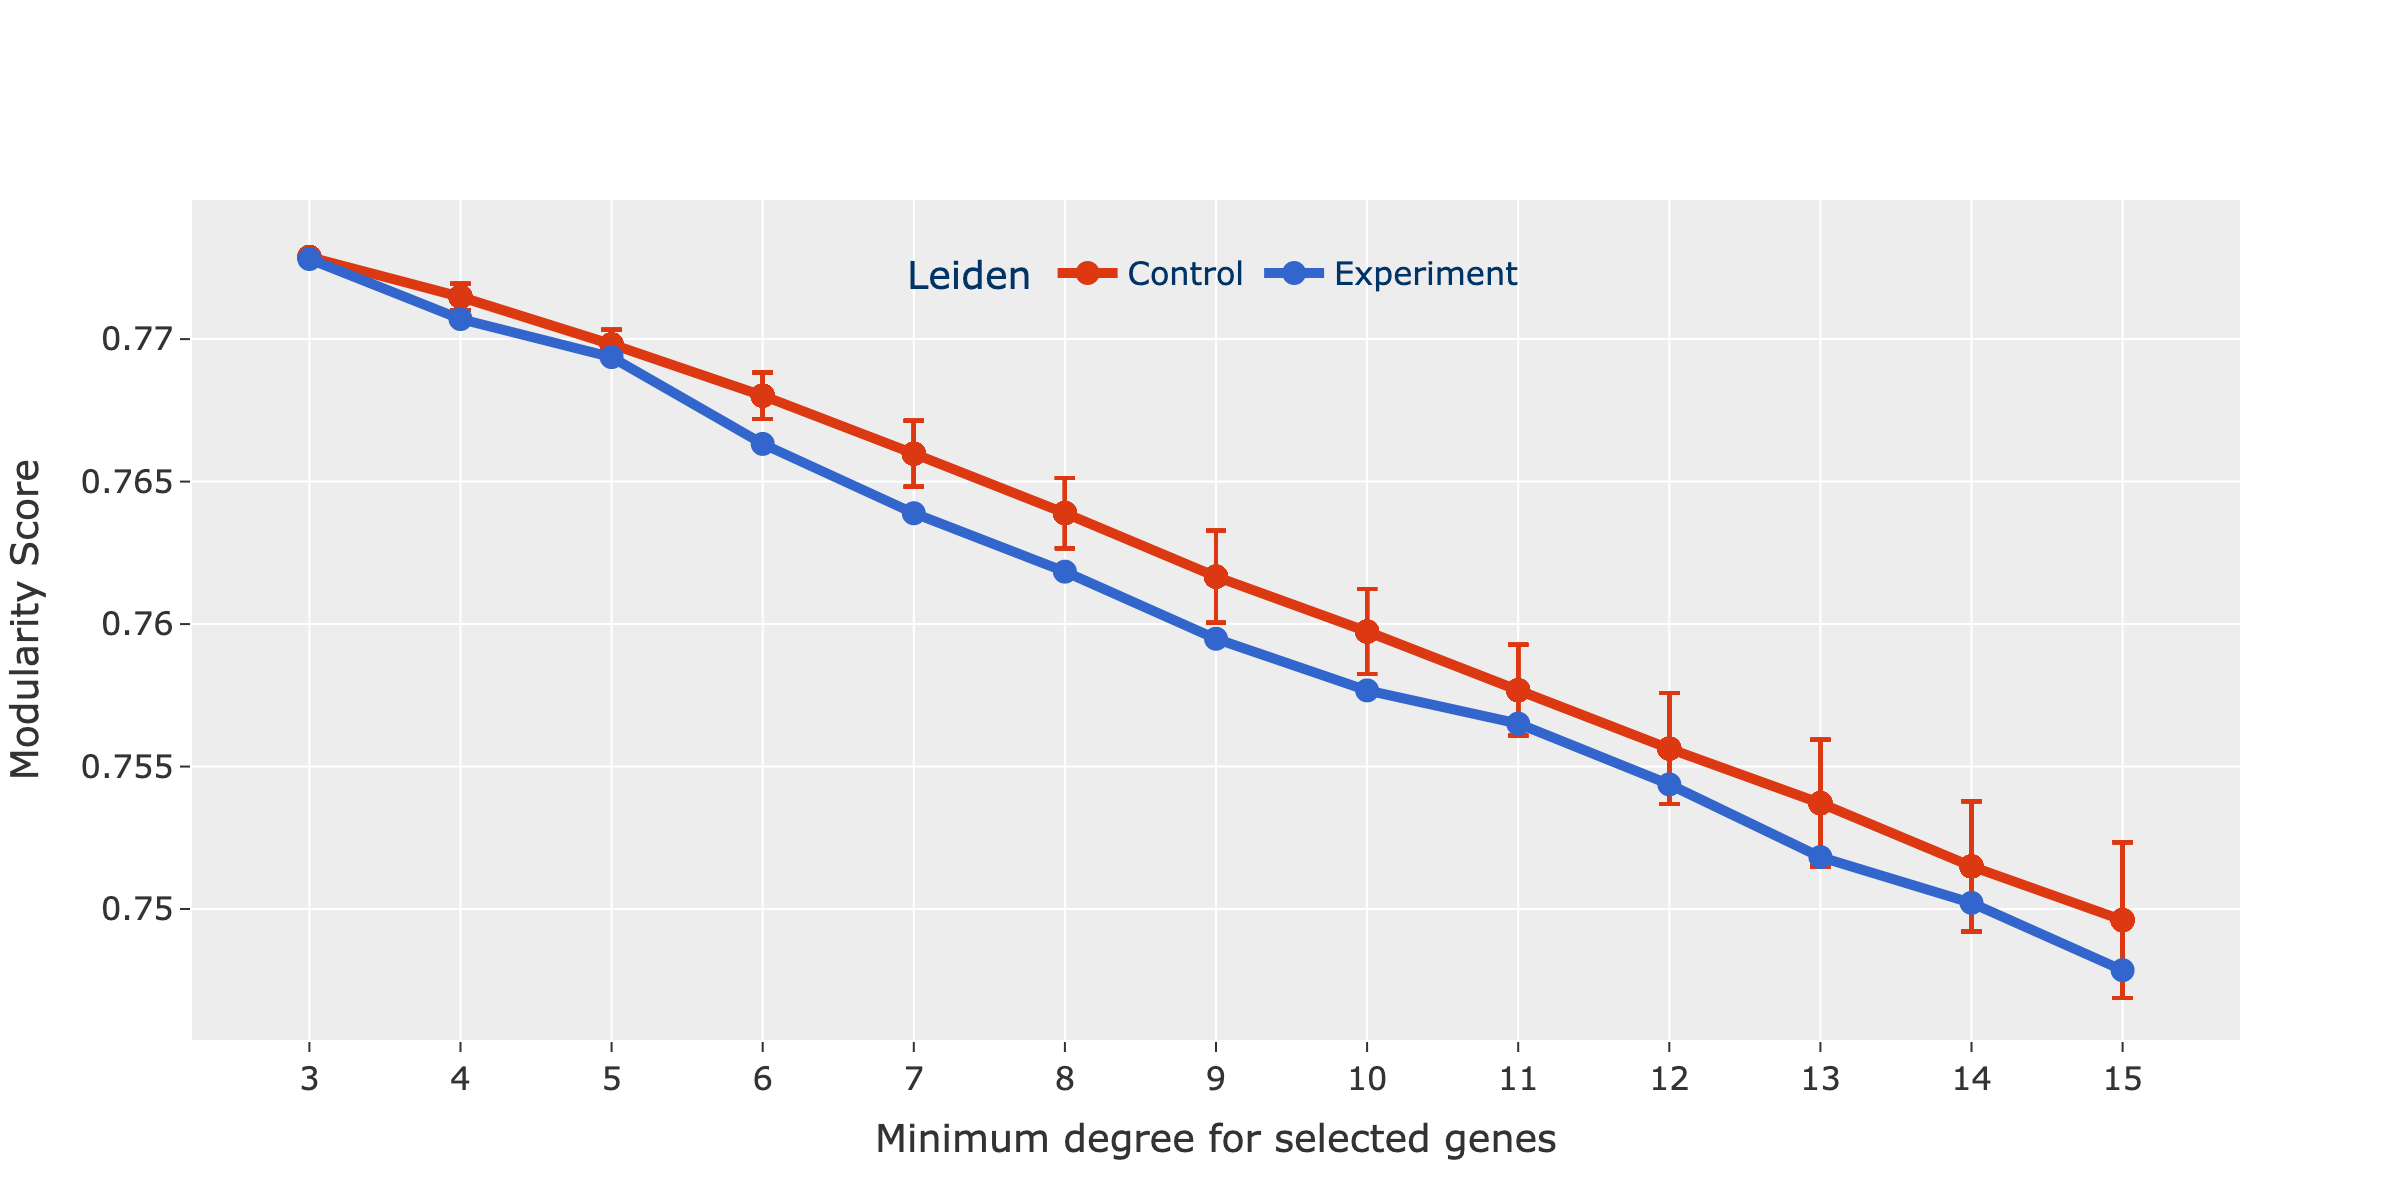
\includegraphics[width=\linewidth]{Sections/Network_I/Resources/selective_pruning/leid_mod_sel_prun.png}
        \caption{Leiden Modularity Maximisation}
    \end{subfigure}\hspace{\fill} % maximize horizontal separation

    \caption{Comparison of the SBM and Leiden}
    \label{fig:N_I:gene_sel}
\end{figure}



\subsubsection{Selected TFs}


\begin{figure}[!ht]   
\centering
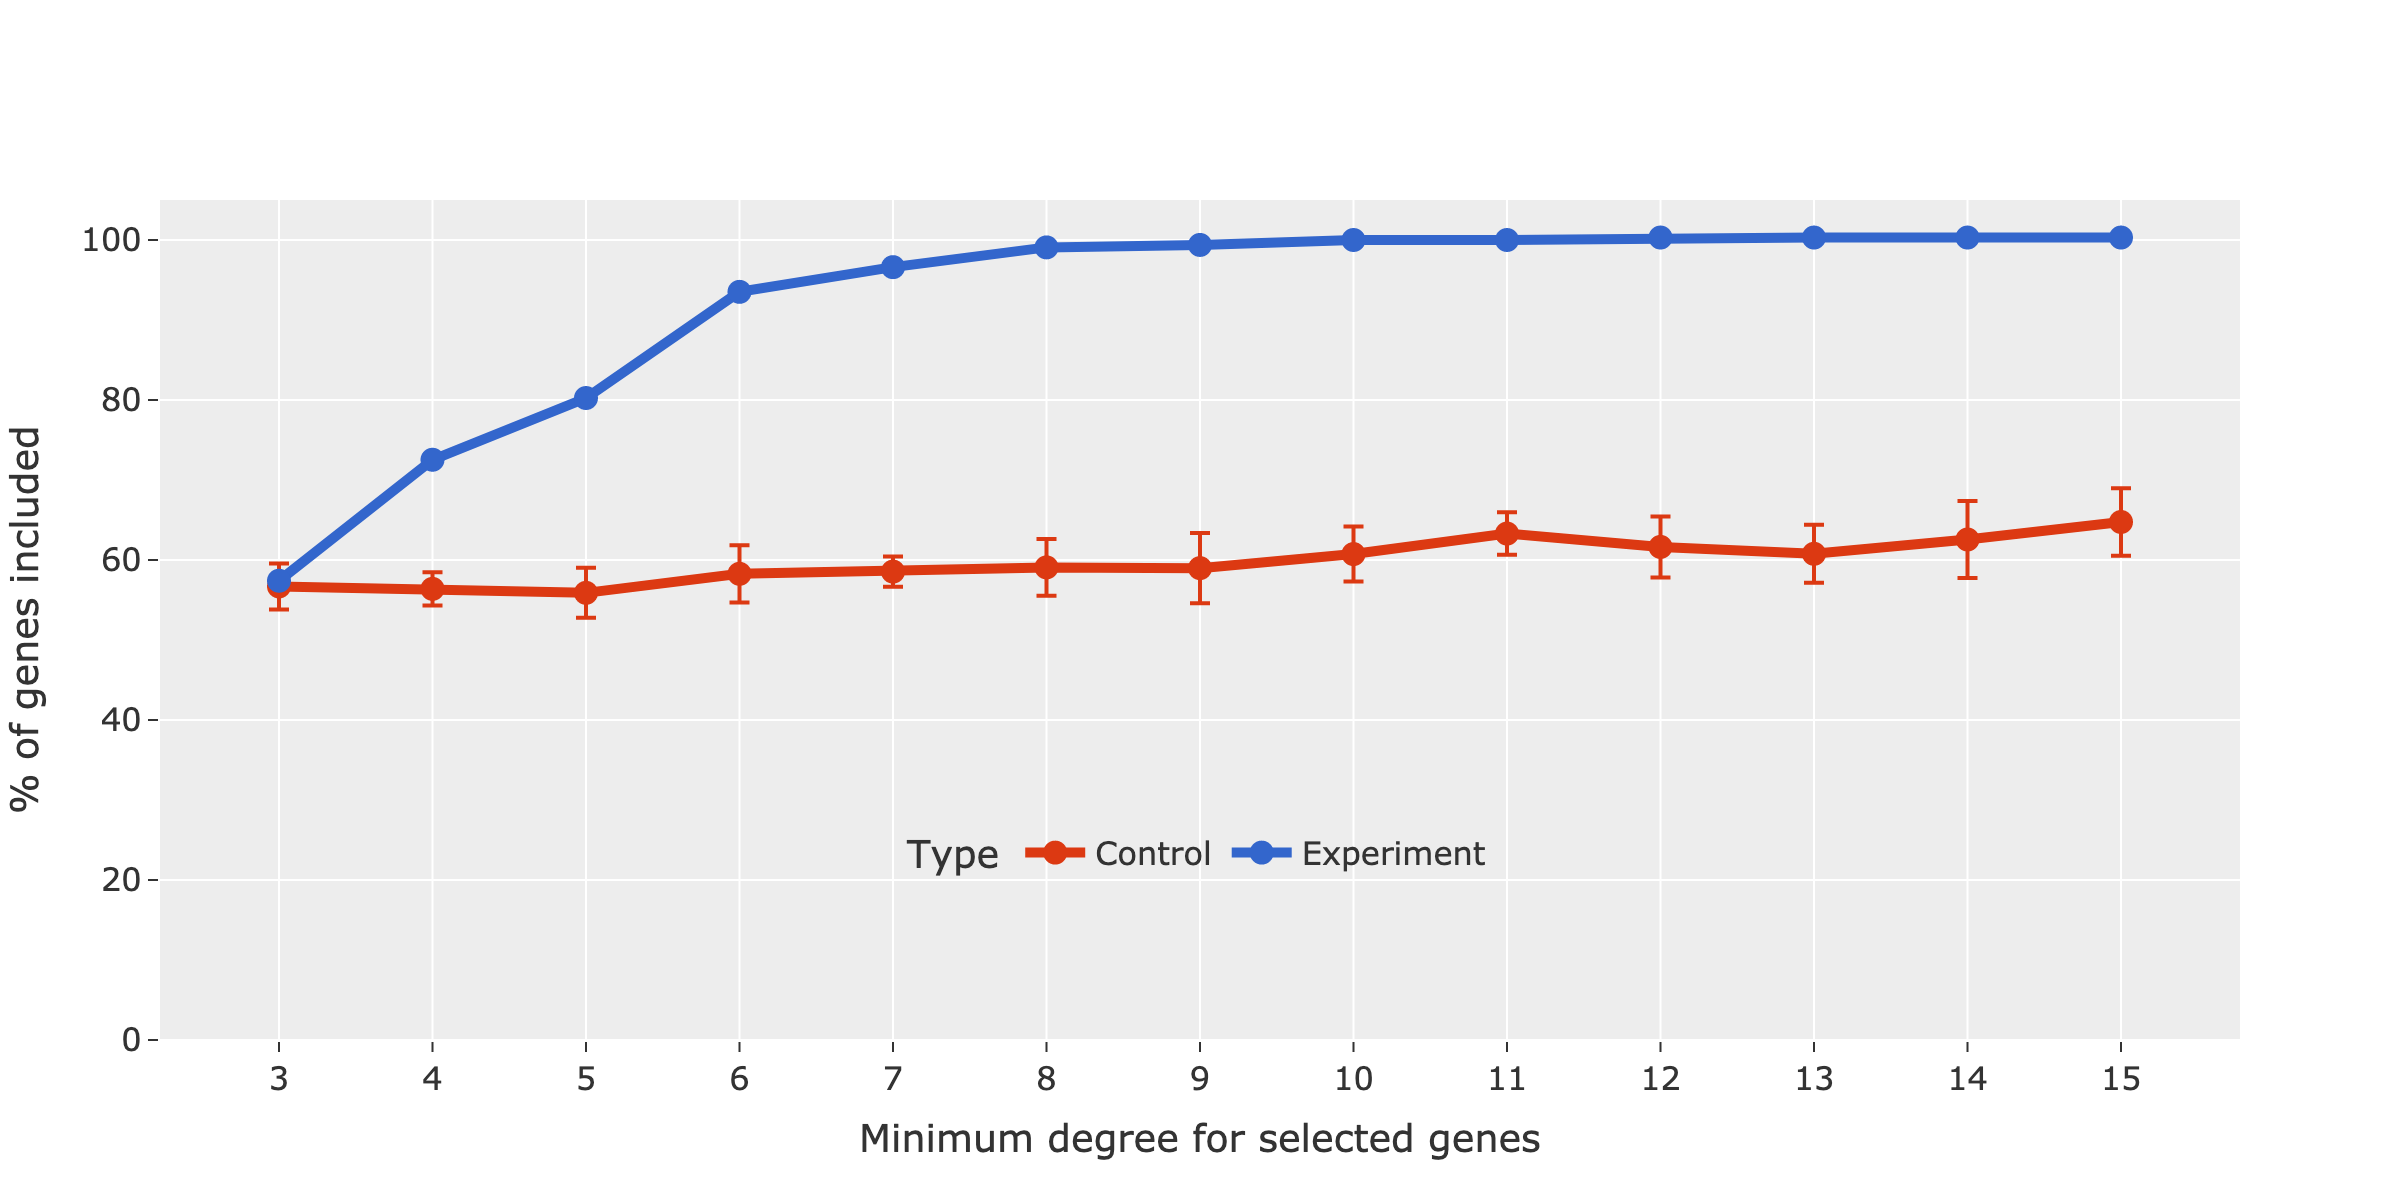
\includegraphics[width=1.0\textwidth,height=1.0\textheight,keepaspectratio]{Sections/Network_I/Resources/selective_pruning/ctrls_min_dig_mev.png}
  \caption{Selected TFs}
\label{fig:N_I:sel_tfs}
\end{figure}


\newpage

\subsubsection{Biological analysis}



\subsubsection{ToDo}

\begin{itemize}
    \item Introduction
    \begin{todolist}
        \item [\done] Why are we doing the experiments? - Because we want to study of the effect of the TF in the network
        \item [\done] What are the experiments performed?
        \item [\done] Community detection comparison
        \item [\done] Which dataset?
        \item [\done] How was the gene selection is done - v3 mostly
        \item [\done] Mention that some of the work done here was presented at the Complex Network conference 
    \end{todolist}
    \item General stats 
    \begin{todolist}
        \item Talk about the TF and how these are present in the dataset
        \item In the cancerous and non-cancerous dataset
        \item Introduce the Human Transcription Factor list and why we want to prioritise them
        \item Show some plots about their mutation count, mean expression
        \item How many these are in the top 5000 genes
    \end{todolist}
    \item Experiments 
    \begin{todolist}
        \item Using the tumour dataset as a starting point as the P0 wasn't that useful
        \item Using SBM for a change from Modularity Class - Comparing the methods
        \item Community size vs Modularity score
        \item Choosing control TFs 
        \item Range for 3-15 - Why choosing this range - all genes are selected by TF
    \end{todolist}
    \item Biological analysis 
    \begin{todolist}
        \item The DEA
        \item Morpheus - clustering
        \item Survival plot
        \item Comparing CS models - can we use this rather then hierarchical clustering
        \item Comparing between subtypes
        \item Significance in terms of the proteins, are those genes find somewhere
    \end{todolist}
    \item Conclusion
    \begin{todolist}
        \item Integration of the TF works
        \item ModCon and MEV selection works 
        \item
    \end{todolist}
\end{itemize}